%Template desenvolvido por Jorge Luiz Ferreira da Silva Junior
%Contato: jorgeluizjk@gmail.com
%Repositório disponível em: https://github.com/Collumbus/Template_Slides_LaTex
%Criado em 18 de julhor de 2018.

\documentclass[aspectratio=169]{beamer}
\usetheme{default} %tema do slide. Tem muitos temas existentes... Gosto desse! Se vcs quiserem mais temas, visitem: http://deic.uab.es/~iblanes/beamer_gallery/index_by_theme.html
\usecolortheme{seagull}
\usepackage[brazil]{babel} %texto
\usepackage[utf8]{inputenc} %texto
\usepackage{graphicx} %imagem	
\usepackage{caption} %imagem
\usepackage{subcaption} %imagem
\usepackage{float} %imagem e tabelas
\usepackage{booktabs} %tabelas	
\usepackage[abnt-emphasize=bf,alf]{abntex2cite} %citacoes ABNT
\usepackage{textpos}  
%Define local da pasta de figuras.  
\graphicspath{{./figuras/}} 		

%Numeração de slides e footnotes
%Opção 1
\usepackage{beamer/themes/outer/beamerouterthemeumbcfootline}
%Opção 2
%\useoutertheme{infolines}

%Insere um plano de fundo: Barra verde
\setbeamertemplate{background canvas}{
\includegraphics
	[width=\paperwidth,height=\paperheight]{bkg.jpg}}

%Insere as Logos

%Logo superior esquerda 1
\addtobeamertemplate{headline}{}{%
	\begin{textblock*}{100mm}(.030\textwidth,0.2cm)
		
\includegraphics[width=1cm]{logo2} 
\end{textblock*}}

%Logo superior esquerda 2
\addtobeamertemplate{headline}{}{%
	\begin{textblock*}{100mm}(.915\textwidth,0.1cm)
		
\includegraphics[width=1.0cm]{logo3} 
\end{textblock*}}

%Logo superior direita 1
\addtobeamertemplate{headline}{}{%
	\begin{textblock*}{100mm}(.110\textwidth,0.17cm)
		
\includegraphics[width=1cm]{logo4}
\end{textblock*}}


%Defini uma cor personalizada
\definecolor{mygreen}{rgb}{.125,.5,.25}
%\usecolortheme[named=mygreen]{structure}

%Customiza marcadores
%\setbeamertemplate{items}[ball]
\setbeamertemplate{itemize item}{\color{mygreen}$\blacksquare$}
\setbeamertemplate{itemize subitem}{\color{mygreen}$\blacktriangleright$}

%Centraliza o título dos slides
\setbeamertemplate{frametitle}[default][center]


%Reservados para o sistema - Não alterar
\title[\imprimirTitulo]{\imprimirTitulo}
\author[\imprimirEmail]{}
\date[]{}
\institute[\imprimirInstituicao]{}
\newcommand{\Autor}[1]{\def\imprimirAutor{#1}}
\newcommand{\Email}[1]{\def\imprimirEmail{#1}}
\newcommand{\Orientador}[1]{\def\imprimirOrientador{#1}}
\newcommand{\Coorientador}[1]{\def\imprimirCoorientador{#1}}
\newcommand{\Data}[1]{\def\imprimirData{#1}}
\newcommand{\Local}[1]{\def\imprimirLocal{#1}}
\newcommand{\Titulo}[1]{\def\imprimirTitulo{#1}}
\newcommand{\Instituicao}[1]{\def\imprimirInstituicao{#1}}
\Autor{Nome do autor}
\Email{email@email.com}
\Orientador{Nome do orientador}
\Coorientador{Nome do coorientador}
\Instituicao{UnB/FGA}
\Titulo{Título do trabalho}
\Data{09 de Agosto de 2018}
\Local{Brasília}


\begin{document}
	

%---------------------------------------------------------------------------
% SLIDE CAPA
%---------------------------------------------------------------------------
	\begin{frame}	
		%Cabeçalho
		\frametitle{\tiny  \textbf{Universidade de Brasília – UnB\\Faculdade UnB Gama – FGA\\ \vspace{0.8mm} Mestrado em Engenharia Biomédica\\ \qquad}}
		\titlepage
		
		%Autor / Orientador
		\begin{textblock*}{100mm}(.35\textwidth,-2.5cm)
			\begin{flushright}
				\footnotesize
				Autor: \imprimirAutor\\
				Orientadora: \imprimirOrientador\\
				Coorientadora: \imprimirCoorientador
			\end{flushright}
		\end{textblock*}

		%Data
		\begin{textblock*}{50mm}(.3\textwidth,-0.5cm)
			\begin{center}
				\footnotesize
				\imprimirLocal, \imprimirData\\
				\imprimirInstituicao
			\end{center}
		\end{textblock*}

	\end{frame}
	
	\begin{frame}
		\frametitle{Sum\'{a}rio}
		\tableofcontents%[pausesections]
	\end{frame}
	
%---------------------------------------------------------------------------
	% PRIMEIRA SECAO
	\section{Imagem}
%---------------------------------------------------------------------------

	% SLIDE 1 - APENAS UMA IMAGEM	
	\begin{frame}
		\frametitle{Imagem}
		\framesubtitle{Imagens simples}
		Imagine a Figura:
		
		\begin{figure}
			\centering
			\caption{Legenda da figura}
			
			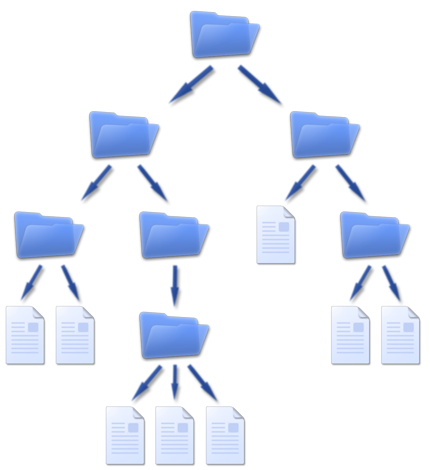
\includegraphics[width=.25\linewidth]{sa.png} 
			
			\footnotesize{Fonte: ...	
				\par Visitado em \today.}
			\label{im1}
		\end{figure}	
	\end{frame}
	
	% SLIDE 2 - APENAS UMA IMAGEM	
	\begin{frame}
		\frametitle{Imagem}
		\framesubtitle{Imagens simples sem legenda}
			Imagine a Figura:
		
			\center
			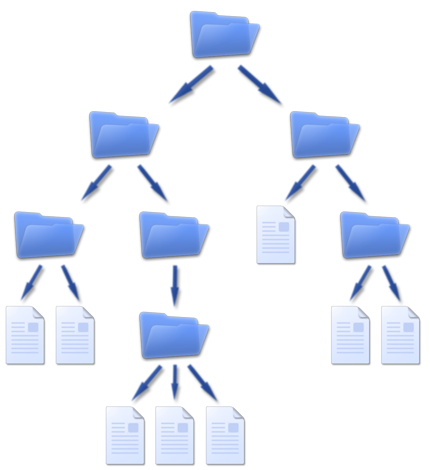
\includegraphics[width=.25\linewidth]{sa.png} 	
	\end{frame}
	
	% SLIDE 3 - TEXTO SEGUIDO DE UMA IMAGEM	
	\begin{frame}
		\frametitle{Imagem}
		\framesubtitle{Imagens agrupadas}
		Imagine a Figura:
		
		\begin{figure}[H]
			\centering
			\caption{Legenda da figura}
			\begin{subfigure}{0.45\textwidth}
				\centering
				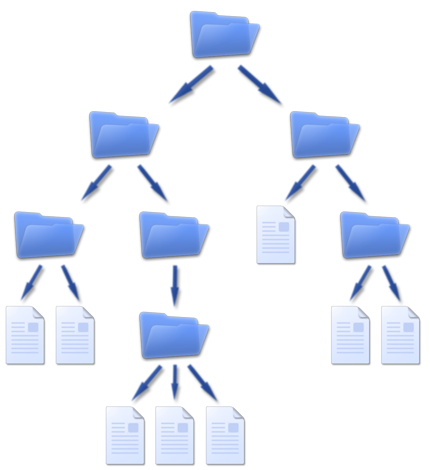
\includegraphics[width=.25\linewidth]{sa.png}
				\caption{Legenda da parte 1}
				\label{figPt1}
			\end{subfigure}
			\hfill
			\begin{subfigure}{0.45\textwidth}
				\centering
				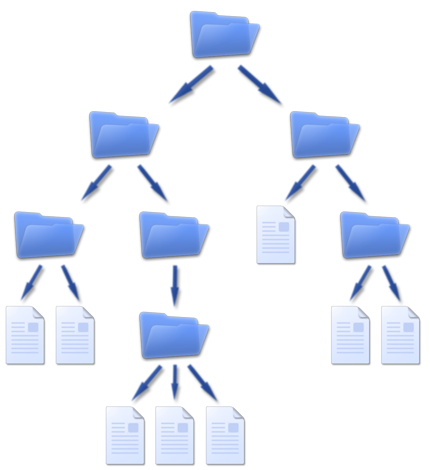
\includegraphics[width=.25\linewidth]{sa.png}
				\caption{Legenda da parte 2}
				\label{figPt2}
			\end{subfigure}                                                   
			
			\footnotesize{Fonte: \citeonline{tanebaun2010}}
			\label{figPt1e2}
		\end{figure}	
	\end{frame}
	
	% SLIDE 4 - TEXTO EM UMA COLUNA, IMAGEM EM OUTRA COLUNA	
	\begin{frame}
		\frametitle{Imagem}
		\framesubtitle{Imagem e texto}
		
		\begin{minipage}[H]{.5\textwidth}
			Texto texto texto texto texto texto texto texto texto texto texto texto texto texto texto texto texto texto texto texto texto texto texto texto texto texto texto texto texto texto texto texto texto texto texto texto texto texto texto texto texto texto texto texto texto texto texto texto texto texto texto texto texto texto texto texto texto texto texto texto texto texto texto texto texto texto texto texto texto texto texto texto texto texto texto texto texto texto texto texto texto texto texto texto texto texto texto.	
		\end{minipage}
		\hfill
		\begin{minipage}[H]{.45\textwidth}
			\begin{figure}
				\centering
				\caption{Legenda da imagem}
				
				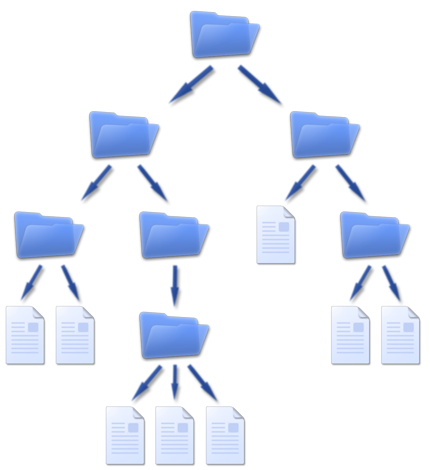
\includegraphics[width=.25\linewidth]{sa.png}
				
				\footnotesize{Fonte: \citeonline{tanebaun2010}}
				\label{figtextimg}
			\end{figure}  
		\end{minipage}
	\end{frame}
	
%---------------------------------------------------------------------------
	% SEGUNDA SECAO
	\section{Tabelas}	
%---------------------------------------------------------------------------
	% SLIDE 5 - UMA TABELA	
	\begin{frame}
		\frametitle{Tabelas}
				
		\begin{table}[H]
			\centering
			\caption{Atributos dos arquivos}
			\begin{tabular}{c|c}
				\toprule
				\textbf{Atributo} & \textbf{Significado} \\
				\midrule
				Prote\c{c}\~{a}o&Quem tem acesso ao arquivo e de que modo\\
				\midrule
				Senha&Necessidade de senha para acesso ao arquivo\\
				\midrule
				Criador&ID do criador do arquivo\\
				\midrule
				Propriet\'{a}rio&Propriet\'{a}rio atual\\
				\bottomrule
			\end{tabular}
			
			\label{tab:attI}
			\footnotesize{Fonte: \citeonline{tanebaun2010}}				
		\end{table}
	\end{frame}
	
%---------------------------------------------------------------------------
	% TERCEIRA SECAO
	\section{Listas}
%---------------------------------------------------------------------------
	% SLIDE 6 - LISTAGEM SIMPLES
	\begin{frame}
		\frametitle{Listas}
		\framesubtitle{Listas Simples}
		\begin{itemize}
			\item \textit{Create};
			\item \textit{Delete};
			\item \textit{Open};
			\item \textit{Close};
			\item \textit{Read};
		\end{itemize}
	\end{frame}
	
	% SLIDE 7 - LISTAS E SUBLISTAS
	\begin{frame}
		\frametitle{Listas}
		\framesubtitle{Listas e sublistas}
		\begin{itemize}
			\item \textit{Create};
			\begin{itemize}
				\item \textit{Open};
				\item \textit{Close};
				\item \textit{Read};
			\end{itemize}
			\item \textit{Delete};
			
		\end{itemize}
	\end{frame}
	
%---------------------------------------------------------------------------
	%SECAO DE REFERENCIAS
	\section{Refer\^{e}ncias bibliogr\'{a}ficas}
%---------------------------------------------------------------------------
	% SLIDE 8 - REFERENCIAS
	\begin{frame}
		\frametitle{Refer\^{e}ncias bibliogr\'{a}ficas indiretas}
		\textbackslash citeonline\{labelDaReferencia\}\\
		\textbf{Resultado}: De acordo com \citeonline{tanebaun2010}, os computadores...
	\end{frame}
		
	% SLIDE 9 - REFERENCIAS
	\begin{frame}
		\frametitle{Refer\^{e}ncias bibliogr\'{a}ficas diretas}
		\textbackslash cite[p. \~{}45]\{labelDaReferencia\} \\
		\textbf{Resultado}: "os computadores..." \cite[p.~45]{tanebaun2010} 
	\end{frame}	

	% SLIDE 10 - REFERENCIAS
	\begin{frame}
		%[allowframebreaks]
		\frametitle{Refer\^{e}ncias bibliogr\'{a}ficas}
		\bibliography{Referencias}
	\end{frame}
	%---------------------------------------------------------------------------
\end{document}
